\chapter{Methodology}\label{chap:method}

\section{Proposed Solution}

Building on the work of Gordillo et al. \cite{sgame2020}, our solution addresses key limitations in their approach. While SGAME provides a platform for creating educational video games by integrating SCORM-compliant learning objects, it has notable restrictions. Specifically, the game creation process in SGAME is confined to combining pre-existing games with a predefined set of educational questions across various fields. Additionally, the system’s support for educational content is limited to the Spanish language, significantly restricting its usability for users from diverse linguistic and cultural backgrounds. Furthermore, SGAME's educational content is primarily focused on middle school to high school curricula, leaving a gap in addressing broader educational needs, such as higher education or specialized training.

To overcome these limitations, our tool is designed to give users greater control over the educational content they can incorporate into their games. Unlike SGAME, which ties games to fixed educational fields, our solution allows the same game template to be adapted for different educational contexts. This approach ensures flexibility, enabling instructors to create games tailored to their specific educational needs and in their preferred language. However, we recognize that certain game templates may naturally align better with specific fields, and such constraints will be accounted for to maintain educational and gameplay coherence.

By addressing these limitations, our tool enhances inclusivity and usability while fostering a more customizable and versatile approach to creating educational games. This empowers instructors to provide engaging and context-specific learning experiences.

\section{System Architecture}

To achieve a tool that can be accessed from various devices and platforms, we have opted for a web-based architecture. The instructor will use a portal to create the game and share it via a link, QR code, or game code with the students. The students will be able to access the game from their devices, as the game will run on any device with a web browser.

We also leverage a Backend as a Service (BaaS) in the cloud to store the data of the games created, as shown in Figure \ref{fig:architecture}. For this purpose, we are using Firebase, which allows the data to be stored in the cloud, making the game accessible from anywhere.

The portal is built using Next.js, a React framework that enables server-side rendering. We have developed two game templates: a Space Invaders-like game, created using Unity and hosted on itch.io, and a click-based puzzle game developed using Next.js. More details on these games are provided in the next section.

\begin{figure}
\centering
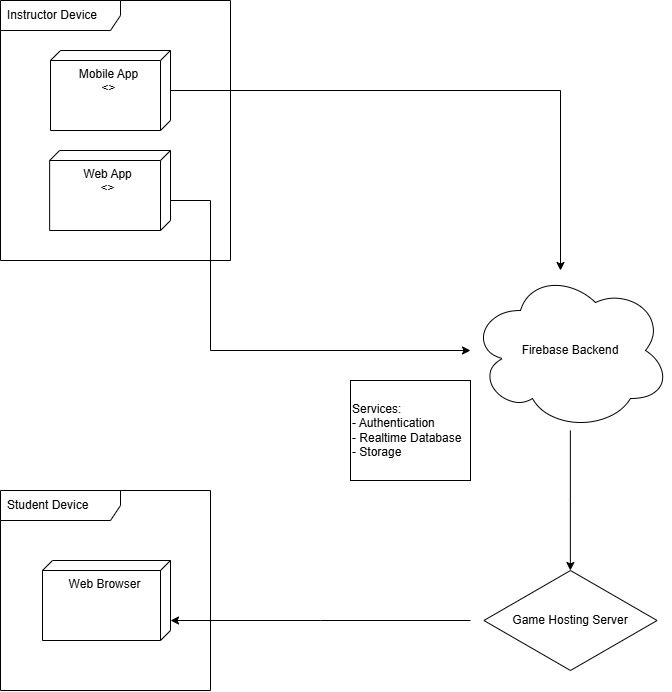
\includegraphics[width=0.8\textwidth]{figures/Deployment_UML.jpg}
\caption{System Architecture}
\label{fig:architecture}
\end{figure}

\section{Instructor Portal}

The instructor portal is a web application that serves as the tool for generating the games. By generating, we mean pushing data to the Firebase Realtime Database. For games like the click-based puzzle game, if an image is required, the image is uploaded to Firebase Storage—at least, that was the original plan. Unfortunately, by the time of implementation, Firebase changed its pricing policy, necessitating a shift to a different storage solution. We opted for Appwrite, an open-source service with a more favorable pricing policy.

After the data is pushed to the database, the portal generates a link, a QR code, and a game code that the instructor can share with the students.

\section{Game Templates}

We have developed two game templates: a Space Invaders-like game and a click-based puzzle game. Both templates are designed to be easily customizable, allowing instructors to add their own educational content.

The Space Invaders-like game is inspired by the classic arcade game, featuring fast-paced gameplay where the player must shoot enemies before they reach the bottom of the screen or hit the player with a projectile. In contrast, the click-based puzzle game offers a more relaxed experience, requiring the player to solve a puzzle by clicking on the correct answer in a provided image.

\subsection{Space Invaders-like Game}

The Space Invaders-like game template allows instructors to incorporate educational content into the fast-paced gameplay. Details on how this template is customized and utilized are discussed further in the implementation section.

\subsection{Click-based Puzzle Game}

The click-based puzzle game template is highly versatile and can be applied to various educational fields, ranging from medicine and engineering to history and geography. In the example provided, the player is tasked with diagnosing a disease by clicking on the correct organ affected.

Using the instructor portal, the instructor uploads an image of the human body and marks the correct organ(s) within defined borders that the player can click on. There can be one or multiple markers, depending on the instructor's choice. The instructor also fills in additional fields such as the patient’s dialog, describing the symptoms, and an extra information field, which provides more context about the condition. Once all fields are completed, the instructor can generate the game and share it with the students.

\begin{figure}
\centering
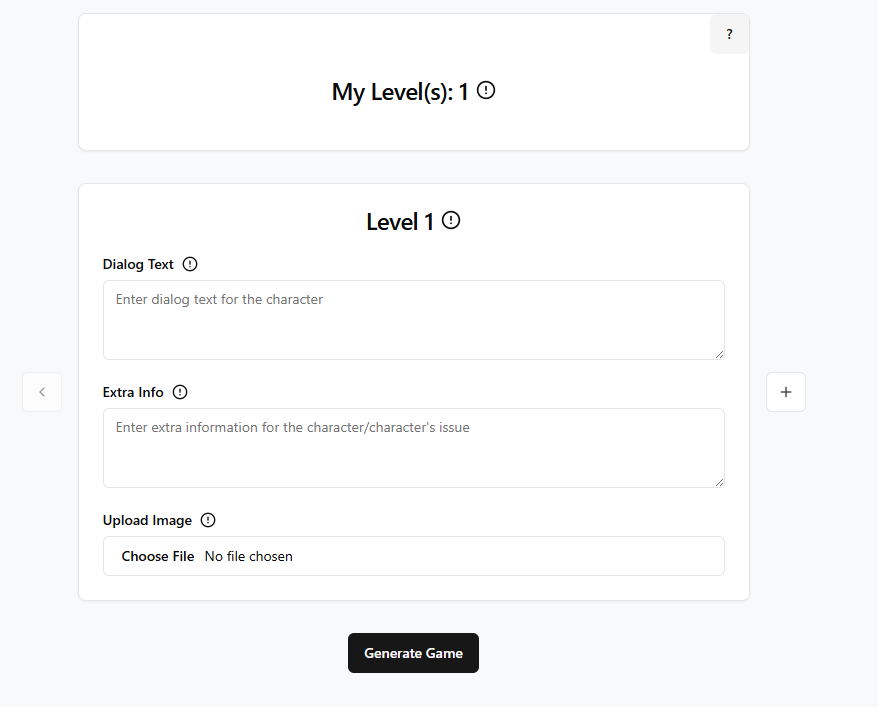
\includegraphics[width=0.49\textwidth]{figures/Diagnose_Game/Instructor_Portal_Diagnose_Game.png}
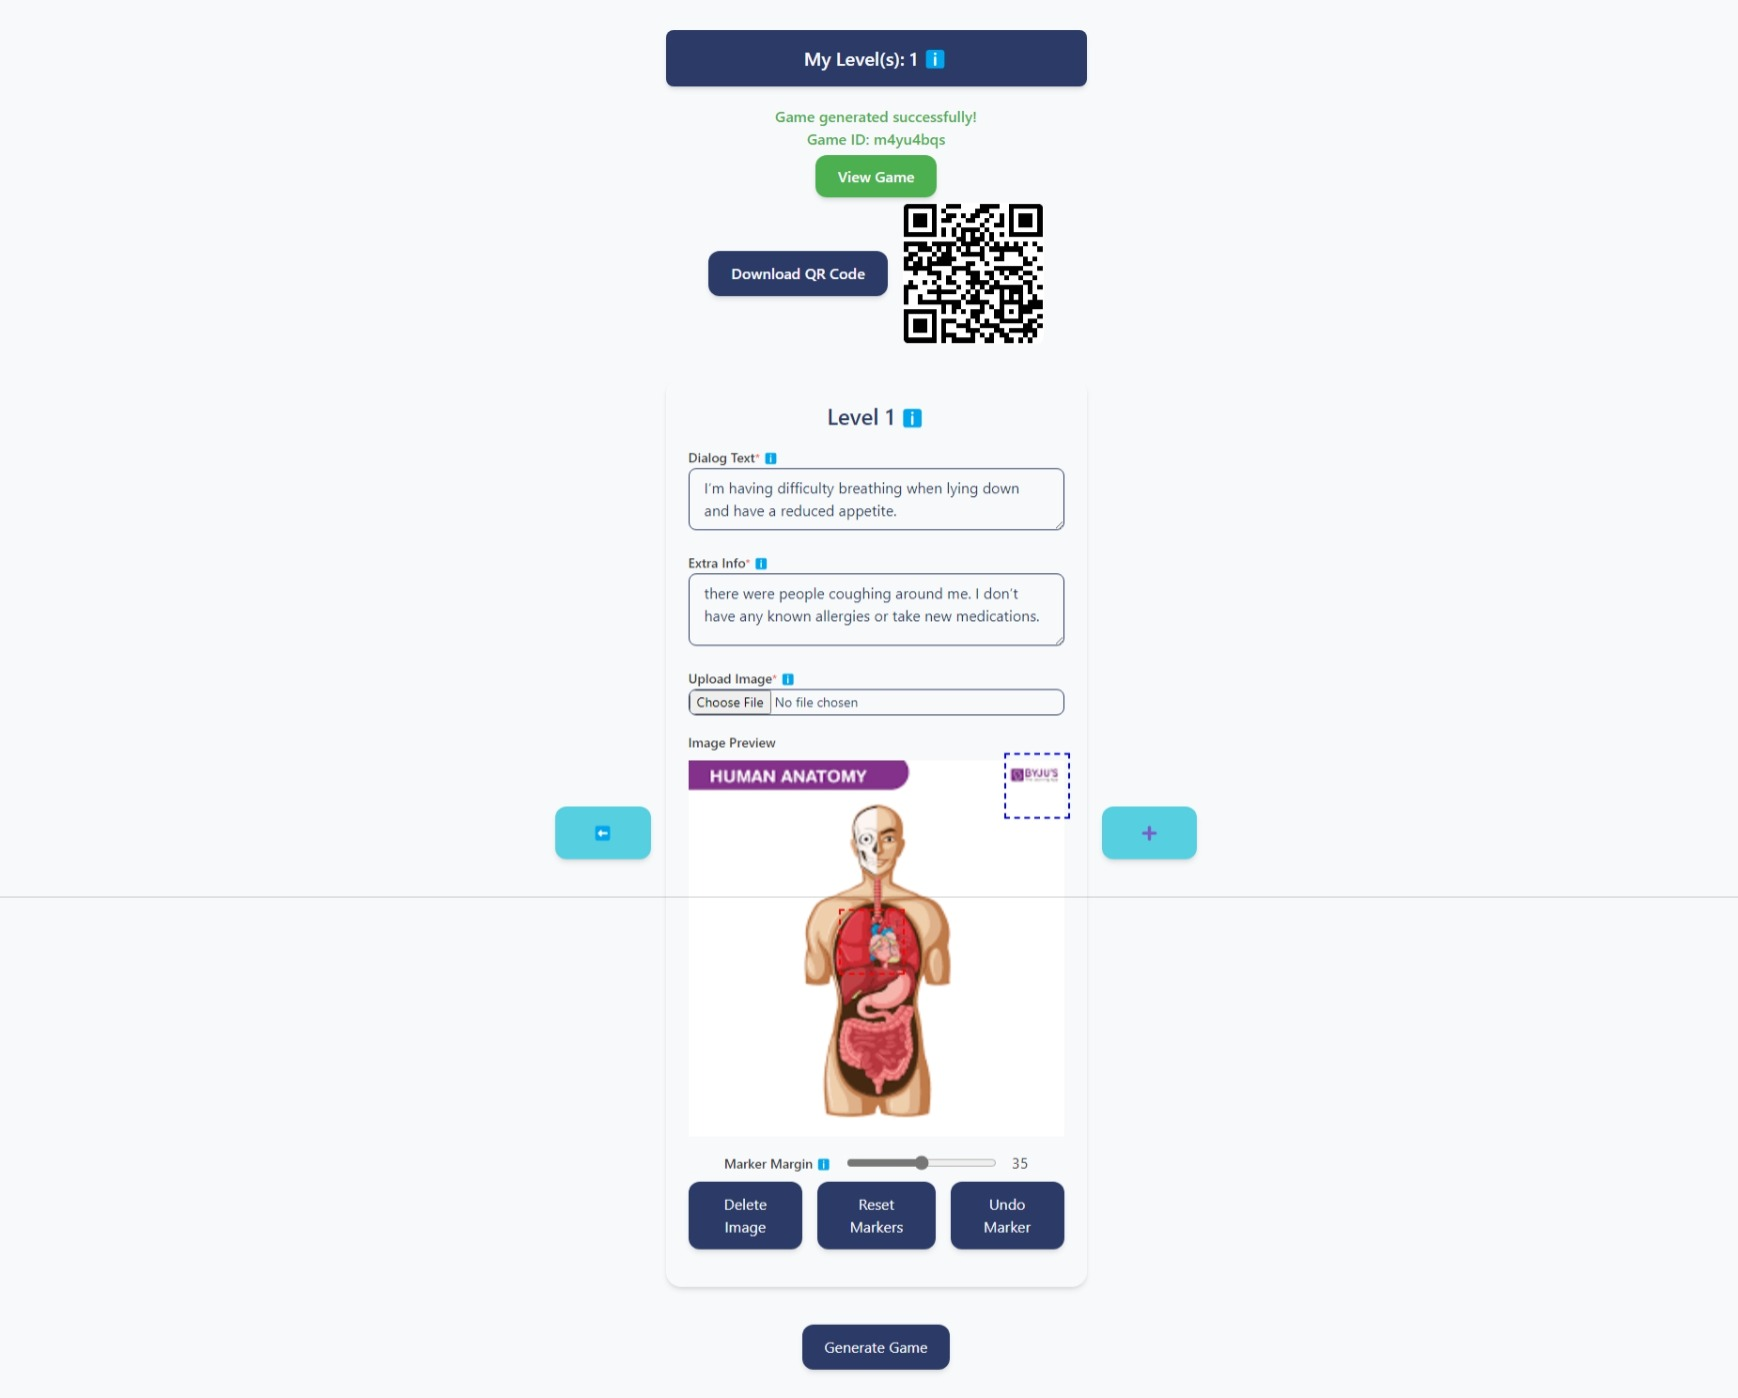
\includegraphics[width=0.49\textwidth]{figures/Diagnose_Game/Instructor_Portal_Diagnose_Game_Generated.jpeg}
\caption{Click-based Puzzle Game: Left - No fields filled; Right - Fields filled and game generated}
\label{fig:click-based-puzzle-game}
\end{figure}